\section{Methodology}
\label{sec:pagestyle}
Let us denote the data by $X \in \real^{N \times P}$ where $N$ is the number of trials  and $P$ is the number of features. $P$ could be $QT$ \textit{i.e.}, the number of sensors $Q$ times the number of time points $T$ if a global threshold has to be computed, or it could be $T$ if only one sensor is considered. To simplify notation, we denote a trial by $X_{i} = (X_{i1}, X_{i2}, ..., X_{iP})$. Also, we define the mean of the trials as  $\overline{X} = \frac{1}{N} \sum_{i=1}^{N} X_{i}$, the median of the trials as $\widetilde{X}$, and the peak-to-peak amplitude of the trials as  $\mathrm{ptp}(X_i) = \mathrm{max}(X_i) - \mathrm{min}(X_i)$.

% -------------------------------------------------------------------------------------
\subsection{Global threshold}
\label{sec:cv_basic}
If we are estimating an optimal global threshold, then $P=QT$ such that the sensor time-series are concatenated across the second dimension of the data matrix. For a fold $k$ (out of total $K$ folds), the data is split into a training set $X_{{train}_{k}}$ and a validation set $X_{{val}_{k}}$ such that ${val}_{k} = [1 .. N] \setminus {train}_{k}$  (see ~\citep{Engemann2015328}) for another use of cross-validation for parameter estimation in the context of M/EEG). The peak-to-peak amplitudes for all trials $X_i$ in the training set is computed as:
\begin{equation}
	\mathcal{A} = \{\mathrm{ptp}(X_i) \suchthat i \in {train}_{k}\}
\end{equation}
Now, let's say we have $L$ candidate global thresholds, $\tau_l \in \real$ for $1 \leq l \leq L$. Then, for one candidate threshold $\tau_l$, the set of indices of the good trials $\mathcal{G}_{l}$ are computed as:
\begin{equation}
\mathcal{G}_{l} = \{i \in {train}_{k} \suchthat \mathrm{ptp}(X_i) < \tau_{l}\}
\end{equation}
The error metric for one fold of the cross-validation for a particular threshold is the Root Mean Squared Error (RMSE) computed as:
\begin{equation}
\label{eq:error_metric}
e_{kl} = \fro{\overline{X}_{\mathcal{G}_{l}} - \widetilde{X}_{val_k}}
\end{equation}
where $\fro{\cdot}$ is the Frobenius norm. The RMSE is computed between the mean of the good trials in the training set $\mathcal{G}_{l}$ with the median of the trials in the validation set. A low rejection threshold will remove too many trials (leading to high RMSE) whereas a high rejection threshold does not remove the bad trials. Cross validation will find an optimal value which is somewhere in between. The median of the trials in the validation set is used to avoid noisy metric values due to outlier trials. This is inspired from literature on robust cross-validation methods ~\citep{leung2005cross, de2003robust} where the loss function is made robust to outlier data.

The threshold with minimum mean error is selected as the global threshold, \textit{i.e.,}
\begin{equation}
\tau_{\star} = \tau_{l_{\star}} \textrm{ with } l_{\star} = \underset{l} \argmin \frac{1}{K} \sum_{k=1}^{K} e_{kl} \enspace .
\end{equation}

We call this method \emph{auto reject (global)}. Note that the threshold learnt this way matches values set manually (Figure~\ref{fig:basic_cv}) and is indeed very different across subjects (Figure~\ref{fig:hist}A).

%-----------------------------------------------------------------------------------
\subsection{Sensor-specific thresholds}
\label{sec:consensus}

\begin{figure}[t]
	\begin{center}
	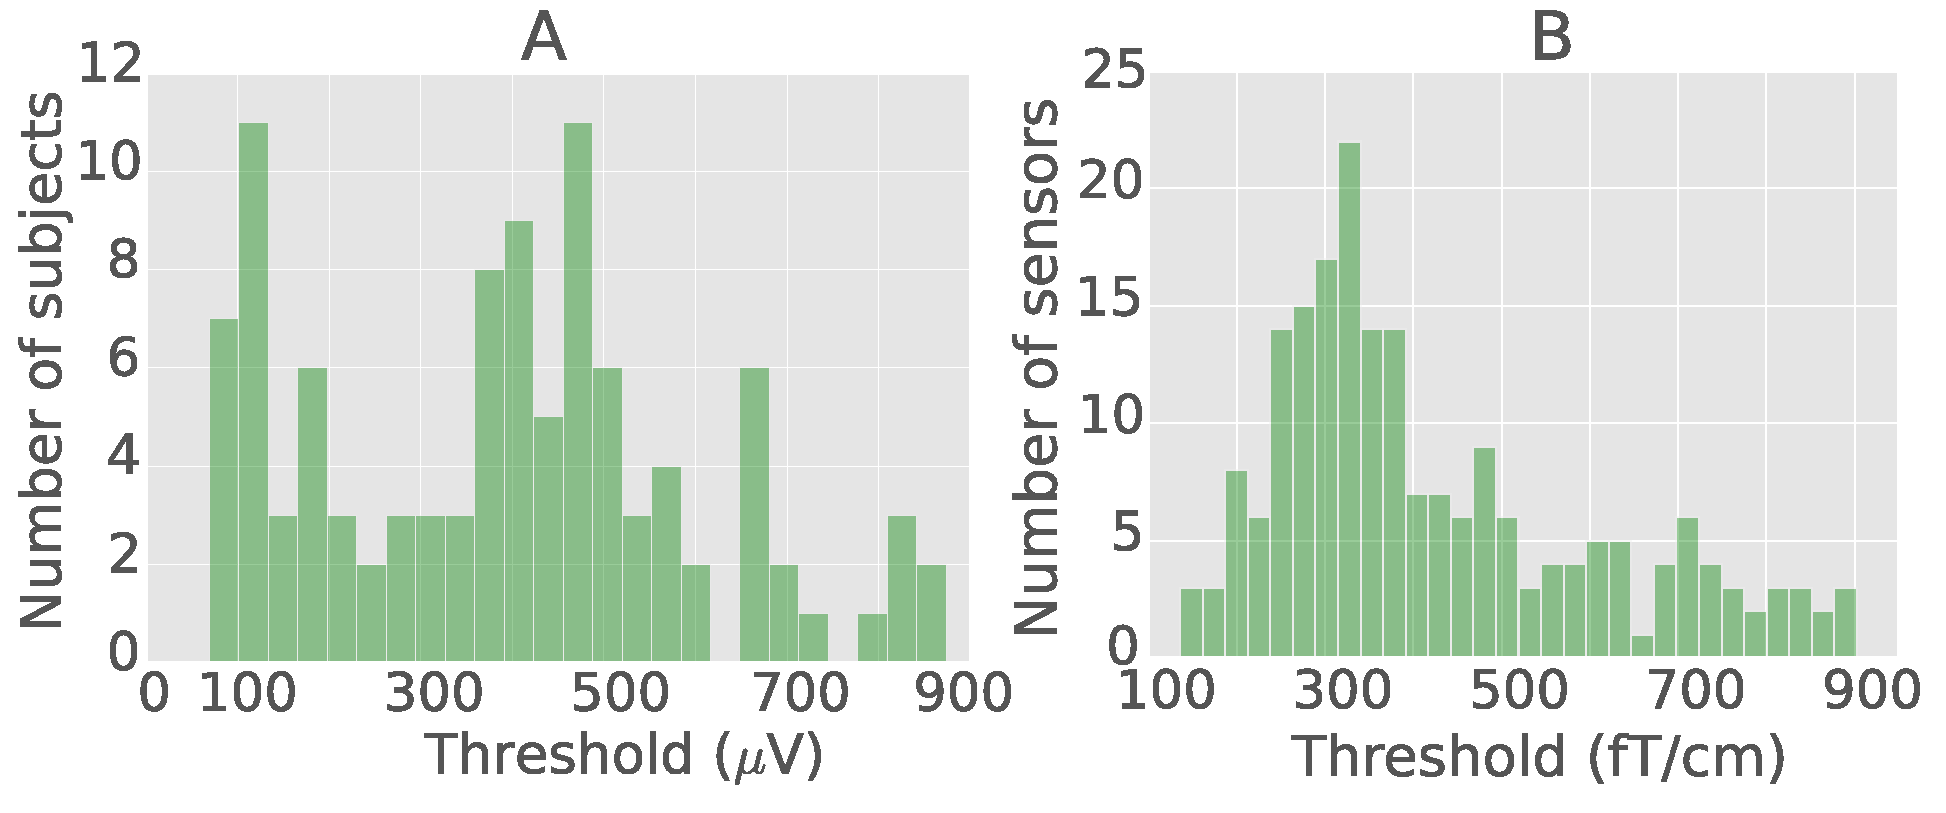
\includegraphics[width=0.8\linewidth]{figures/figure2.pdf}
    \end{center}
    \caption{A. Histogram of thresholds for subjects in the EEGBCI dataset with \emph{auto reject (global)} B. Histogram of sensor-specific thresholds in gradiometers for the MNE sample dataset (Section~\ref{sec:results}). The threshold does indeed depend on the data (subject and sensor).}
    \label{fig:hist}
\end{figure}

In practice however, a global rejection threshold for all sensors is certainly not optimal. Depending on the sensor noise levels and the experiment, each sensor can necessitate a different rejection threshold (Figure~\ref{fig:hist}B). Learning a sensor-specific threshold is what we propose next. With a sensor-specific threshold, each sensor votes whether a trial should be marked as good or bad. If a trial is voted as bad by a minimum number of sensors, then it will be marked as bad. \iftoggle{long}{Voting not only optimizes for sensor-specific thresholds but also allows one sensor to compensate for ``mistakes" made by another sensor.}{}

The cross-validation procedure here is the same as in Section~\ref{sec:cv_basic} except that now $P=T$. For every sensor, one can thus learn a sensor-specific threshold $\tau_{\star}^{q}$ where $q \in [1 .. Q]$. However here these thresholds will not be directly used to drop any trial (Equation~\ref{eq:indicator_matrix} shows how they are used).

For the cross-validation to work, at least some of the sensor data must be clean. However, this is not the case with globally bad sensors. 
% alex's version below
%To obtain a small cross-validation error using \eqref{eq:error_metric}, one needs to average as many good trials as possible. This suggests an automatic selection of not too high thresholds. This is undesirable when a sensor is globally bad with large peak-to-peak values for every trial. 
Therefore, we generate a cleaner copy of each trial by interpolating each sensor from all the others. By doing so, we double the size of the data and generate an augmented matrix $X^{a} \in \real^{2N \times T}$. This augmented matrix is then used for cross validation (as described in Section~\ref{sec:cv_basic}). 
%\iftoggle{long}{If a sensor is globally bad, then the \iftoggle{long}{}{learned} threshold}{} \iftoggle{long}{would be selected such that it}{We then} mark the interpolated data as good and the original data as bad. 
For interpolation, we use the procedure outlined in \citep{hamalainen1994interpreting} for MEG and \citep{perrin1989spherical} for EEG. Both are implemented in MNE-Python \citep{gramfort2013meg} .


%To fix this problem, we \iftoggle{long}{propose to }{}augment the sensor data with data interpolated from data in all the other sensors. \iftoggle{long}{Thus, we have the original trials and the interpolated trials, which we combine}{resulting} in a matrix $X^{a} \in \real^{2N \times T}$. 

Now, let us define an indicator matrix $C \in \{0, 1\}^{N \times Q}$ whose entries $C_{ij}$ are formed according to the rule:
\begin{equation} \label{eq:indicator_matrix}
C_{ij} = \begin{cases} 
0, & \text{if } \mathrm{ptp}(X_{ij}) \leq \tau^{j}_{\star} \\
1, & \text{if } \mathrm{ptp}(X_{ij}) > \tau^{j}_{\star}
\end{cases}
\end{equation}
Each column of this matrix indicates which sensors vote which trials as bad. If the number of sensors which vote a trial as bad exceeds a certain number of sensors $\kappa$, then the trial is marked as bad. That is, we take a consensus among the sensors and mark a trial as bad only if the consensus is high enough. In other words, good trials $\mathcal{G}$ are given by
\begin{equation}
\mathcal{G} = \{i \suchthat \sum_{j=1}^{Q} C_{ij} < \kappa \}
\end{equation}
In practice, we will use $\kappa/Q$ which is a fraction of the total number of sensors to have a parametrization that is as independent as possible from the total number of sensors.

%------------------------------------------------------------------------------------
\subsection{Trial-by-trial interpolation}

\begin{figure}[t]
	\begin{center}
	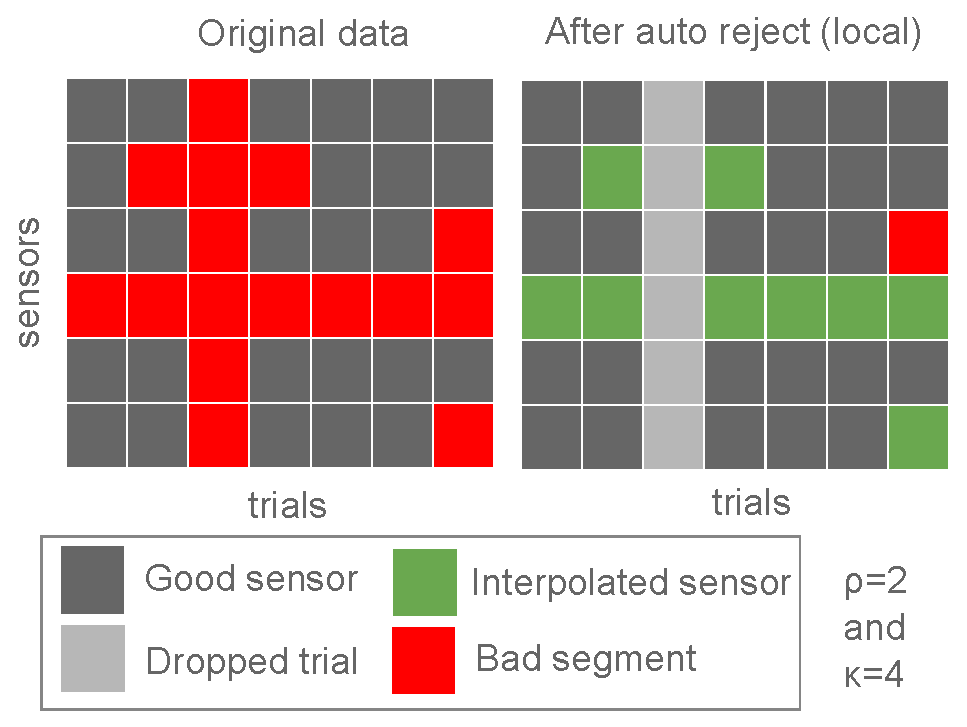
\includegraphics[width=0.7\linewidth]{figures/fig_xx_auto_reject_scheme.pdf}
    \end{center}
    \caption{A schematic explaining how \emph{auto reject (local)} works. \emph{Auto reject (local)} drops the minimal number of sensors and interpolates the rest.}
    \label{fig:schematic}
\end{figure}

Once we find the bad trials by consensus, the next step is to repair the trials which are good but have a limited number of bad sensors. Since these sensors might be bad locally (\textit{i.e.}, bad for only a few trials) or globally (\textit{i.e.}, bad for all trials), we choose to interpolate the sensors trial-by-trial. Note that we cannot interpolate more than a certain number of sensors. This number depends on the data and the total number of sensors present. Therefore, we choose to interpolate only the worst $\rho$ sensors.

For each trial where the number of bad sensors is larger than $\rho$, the bad sensors are ranked based on the peak-to-peak amplitude. The higher the peak-to-peak amplitude, the worse is the sensor. That is, we can assign a score $s_{ij}$ which is $-\infty$ if the sensor is good and equal to the peak-to-peak amplitude if the sensor is bad.

\begin{equation}
s_{ij} = \begin{cases}
-\infty & \text{if } C_{ij} = 0 \\
\mathrm{ptp}(X_{ij}) & \text{if } C_{ij} = 1
\end{cases}
\label{eq:score}
\end{equation}

% The entries of the scoring matrix $S \in \real^{N \times P}$ are computed as the fraction where the peak-to-peak amplitude of the current trial and sensor $X_{ij}$ is lower than the peak-to-peak amplitude of all the augmented trials. More formally:
%
%\begin{equation}
%s_{ij} = \frac{1}{2N} \sum_{r=1}^{2N} [\mathrm{ptp}(X_{ij}) \leq \mathrm{ptp}%(X^{a}_{rj})]
%\end{equation}
%
% where $[\cdot]$ is the Iversion bracket, which is 1 when the condition inside the brackets is satisfied, and 0 otherwise.
This leads us to the following rule for interpolating a sensor $X_{ij}$: 
\begin{equation}
X_{ij} = \begin{cases}
\mathrm{interp}(X_{ij}), & \text{if } (0 < \sum_{j'=1}^{Q} C_{ij'} \leq 
\rho) \\ & \text{and } (C_{ij} = 1)\\ 
\mathrm{interp}(X_{ij}), & \text{if } (\rho < \sum_{j'=1}^{Q} C_{ij'} \leq \kappa) \\ & \text{and } (s_{ij} > s_{i(N-\rho)})\\
X_{ij}, & \text{otherwise}
\end{cases}
\label{eq:auto_reject}
\end{equation}
where the notation $s_{i(k)}$ indicates the k-th order statistic, \textit{i.e.}, the k-th smallest value. $\mathrm{interp(\cdot)}$ is a generic function which interpolates the data. That is, when the number of bad sensors in a trial $\sum_{j=1}^{Q} C_{ij}$ is less than the maximum number of sensors $\rho$ which can be interpolated, they are all repaired by interpolation. However, when this is not the case, only the worst $\rho$ sensors are repaired. \iftoggle{long}{Figure~\ref{fig:schematic} summarizes Equation~\ref{eq:auto_reject} in a schematic diagram.}{}

\begin{figure}[t]
	\begin{center}
	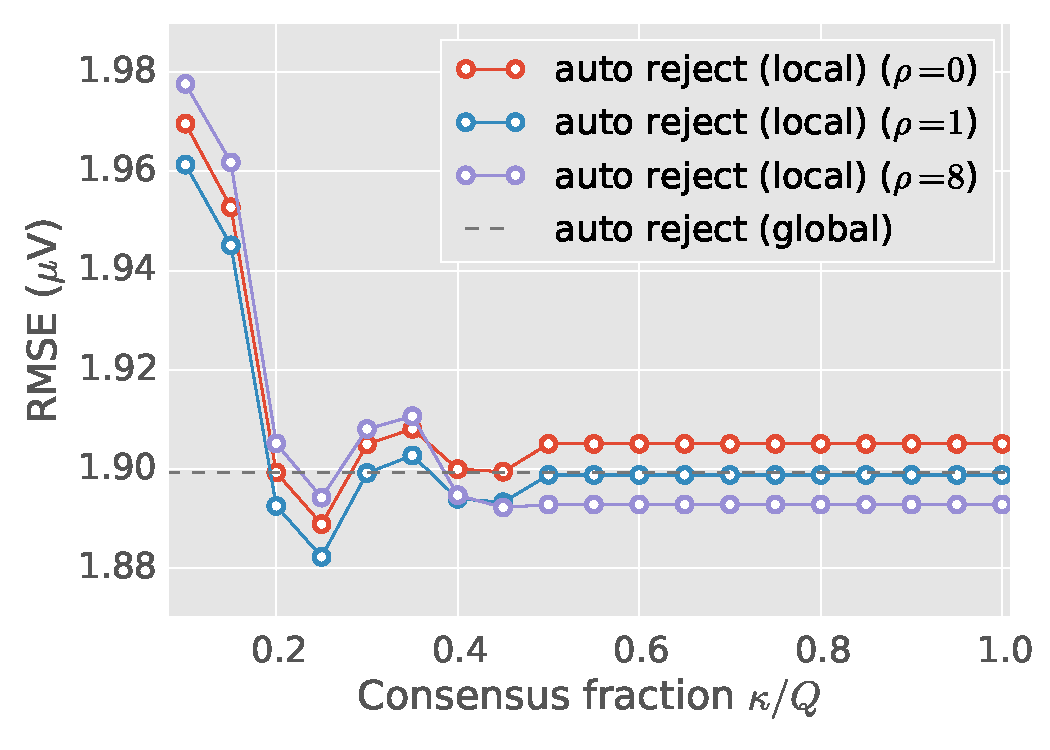
\includegraphics[width=0.7\linewidth]{figures/figure3.pdf}
    \end{center}
    \caption{Root mean squared error (RMSE) for subject 11 in the \emph{Faces} dataset (Section~\ref{sec:results}), averaged over cross-validation folds as a function of minimum fraction of sensors $\kappa / Q$ which must agree for a trial to be marked as bad. The RMSE is plotted for different $\rho$ values. \emph{Auto reject (global)} is the RMSE for using a global threshold to remove trials (Section~\ref{sec:cv_basic}). The best parameters $\rho_{*}$ and $\kappa_{*}$ are those which yield the minimum RMSE.
 }
    \label{fig:fine_reject}
\end{figure}

%----------------------------------------------
% \subsection{Putting it all together}
The optimal values of parameters $\kappa_{\star}$ and $\rho_{\star}$ are estimated using grid search for the same error metric as defined in Equation~\ref{eq:error_metric}. Figure~\ref{fig:fine_reject} shows an example of how the grid search is done for the two parameters. We call this method \emph{auto reject (local)}.
